\documentclass{article}

\usepackage{color}
\usepackage{hyperref}
\usepackage{pdfpages}


\title{\bf Student Krylov Day 2015}
\author{\href{http://sscdelft.github.io/activities/2015/02/02/krylov-day.html}{SIAM Student Chapter Delft}}
\date{February 2, 2015}
\begin{document}
\maketitle
\section*{Prefix}
Krylov subspace methods is an important tool which has been applied successfully to solve different problems 
in the Numerical Algebra. The Netherlands has been a pioneer country in the developing of Krylov method.
Methods like the Conjugate Gradient Squared (CGS), Bi-Conjugate Gradient Stabilized (BiCGSTAB), Nested GMRES (GMRESR), and the Induced Dimension Reduction method (IDR)  
are examples of Krylov methods developed in the Dutch universities. 
We are organizing The Dutch Seminar on Krylov subspace methods with the aim 
to bring together the young researcher to provide an
overview of the state-of-the-art of Krylov subspaces methods and encourage 
the collaboration among them.
\newpage
\section*{Program}
\begin{table}[h]
\begin{tabular}{lll}
10:00 - 10:10 & Reinaldo & Welcoming \\
10:10 - 10:50 & P. Sonnefeld & The story of IDR(s) \\
\hline
11:00 - 11:20 & Manuel & Krylov methods for shifted linear systems \\
11:20 - 11:40 & Xian-Ming & Recent progresses in Krylov subspace methods\\
                        & & for solving complex symmetric linear systems\\
11:40 - 12:00 & Ian & tba\\
\hline
12:00 - 13:30 & & Lunch at TU Delft Sports Center \\
\hline
13:00 - 13:20 & Heiko & Preconditioning of Large-Scale Saddle Point Systems\\
                    & & for Coupled Flow Problems\\
13:20 - 13:40 & J\"orn & A Krylov Subspace Approach to Modeling of \\
                     & & Wave Propagation in Open Domains\\
13:40 - 14:00 & Jing & A conjugate gradient based method for \\
                   & & frictional contact problems\\
\hline
14:30 - 14:50 & Tom{\'a}{\v s} & On the numerical behaviour of the CG method\\
14:50 - 15:10 & Pat & Krylov subspace methods for matrix equations \\
                  & & which include matrix 
functions\\
15:10 - 15:30 & Ana & On Low-rank Updates of Matrix Functions\\
\hline
16:00 - 16:20 & Reinaldo & Induced Dimension Reduction method \\
            & & to solve the Quadratic Eigenvalue Problem \\
16:20 - 16:40 & Mario & Rational Least Squares Fitting using Krylov Spaces\\
16:40 - 17:00 & Sarah & Probabilistic bounds for the matrix condition number \\
                    & & with extended Lanczos bidiagonalization\\
\hline
17:00 - 18:00 & & Snacks \& drinks at TU Delft
\end{tabular}
\end{table}
In the evening we will go to \href{http://www.burgerz.nl/en/contact/delft}{Burgerz} - a nice restaurant close to the main train station. Everybody is welcome to join!
% \newpage
% \section{Book of abstracts}
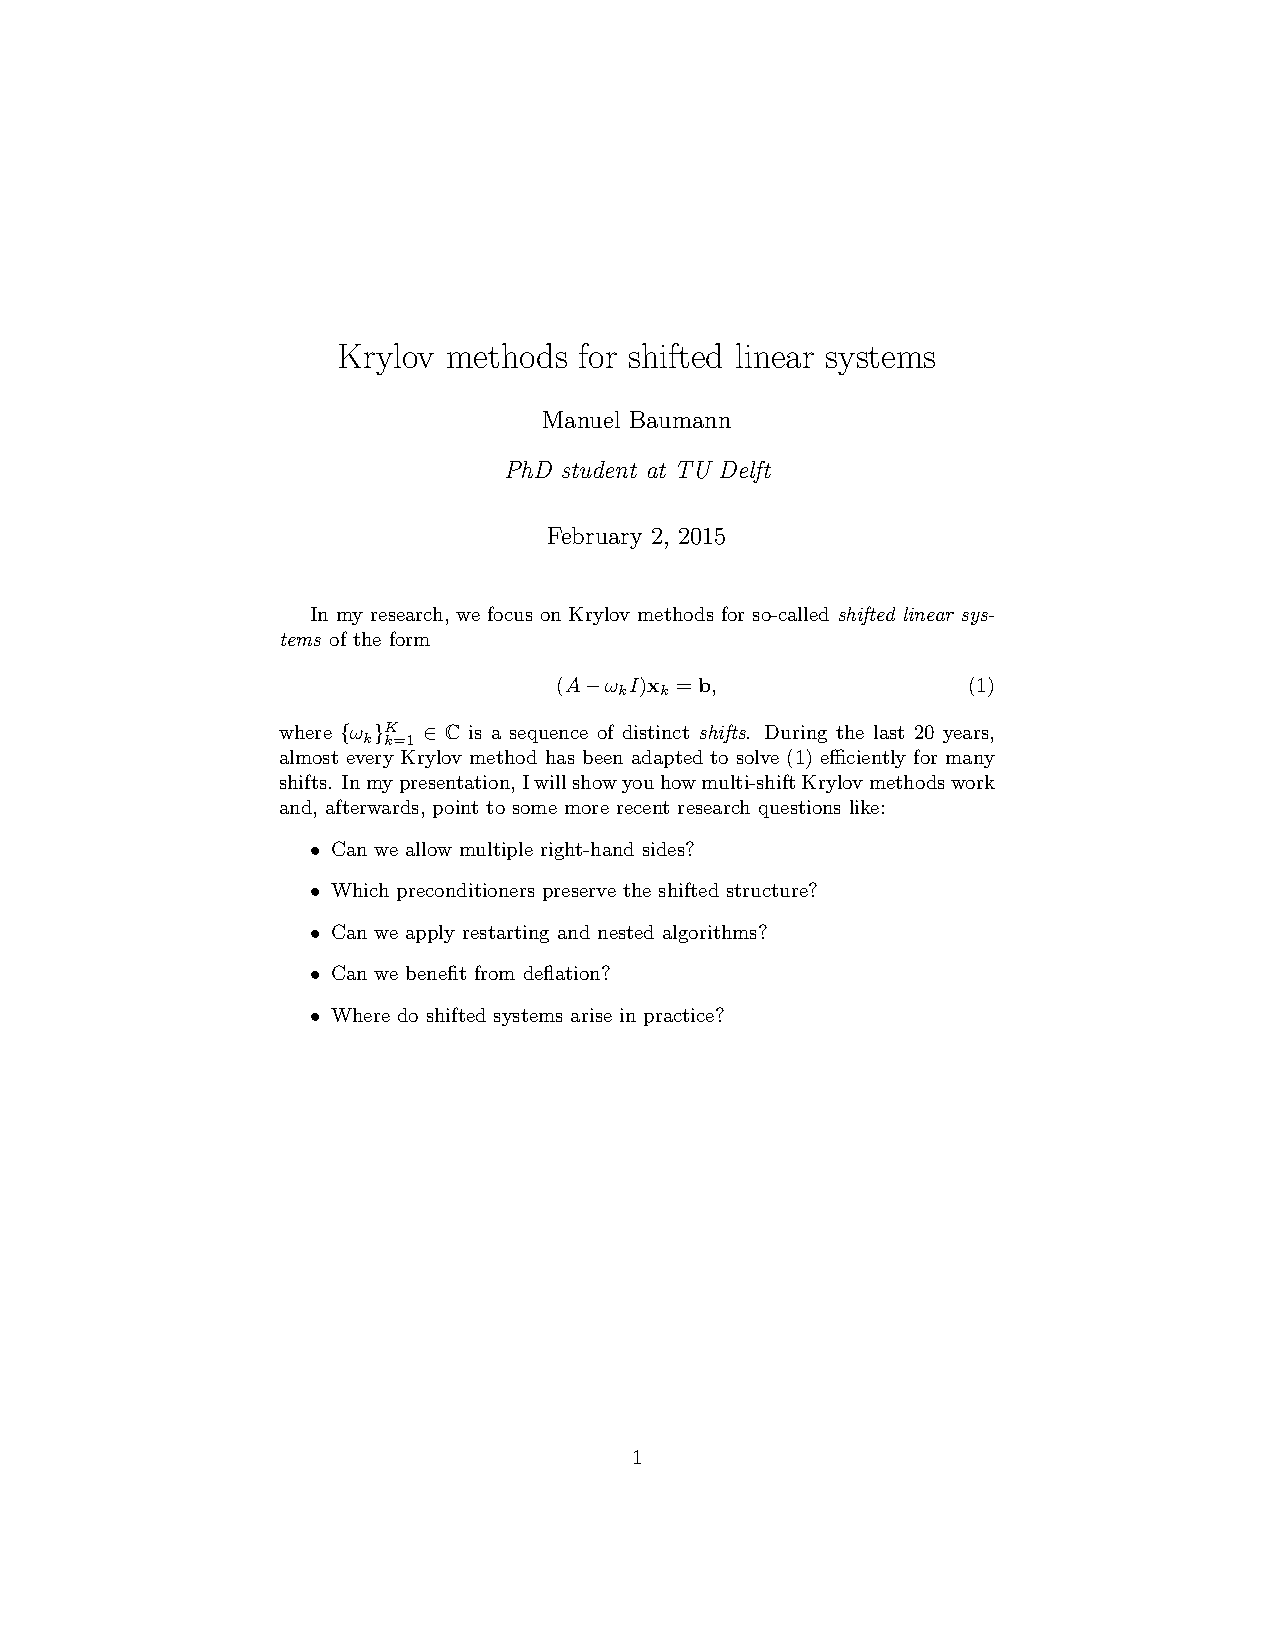
\includepdf[pages={1}]{abstracts/baumann_kd15.pdf}
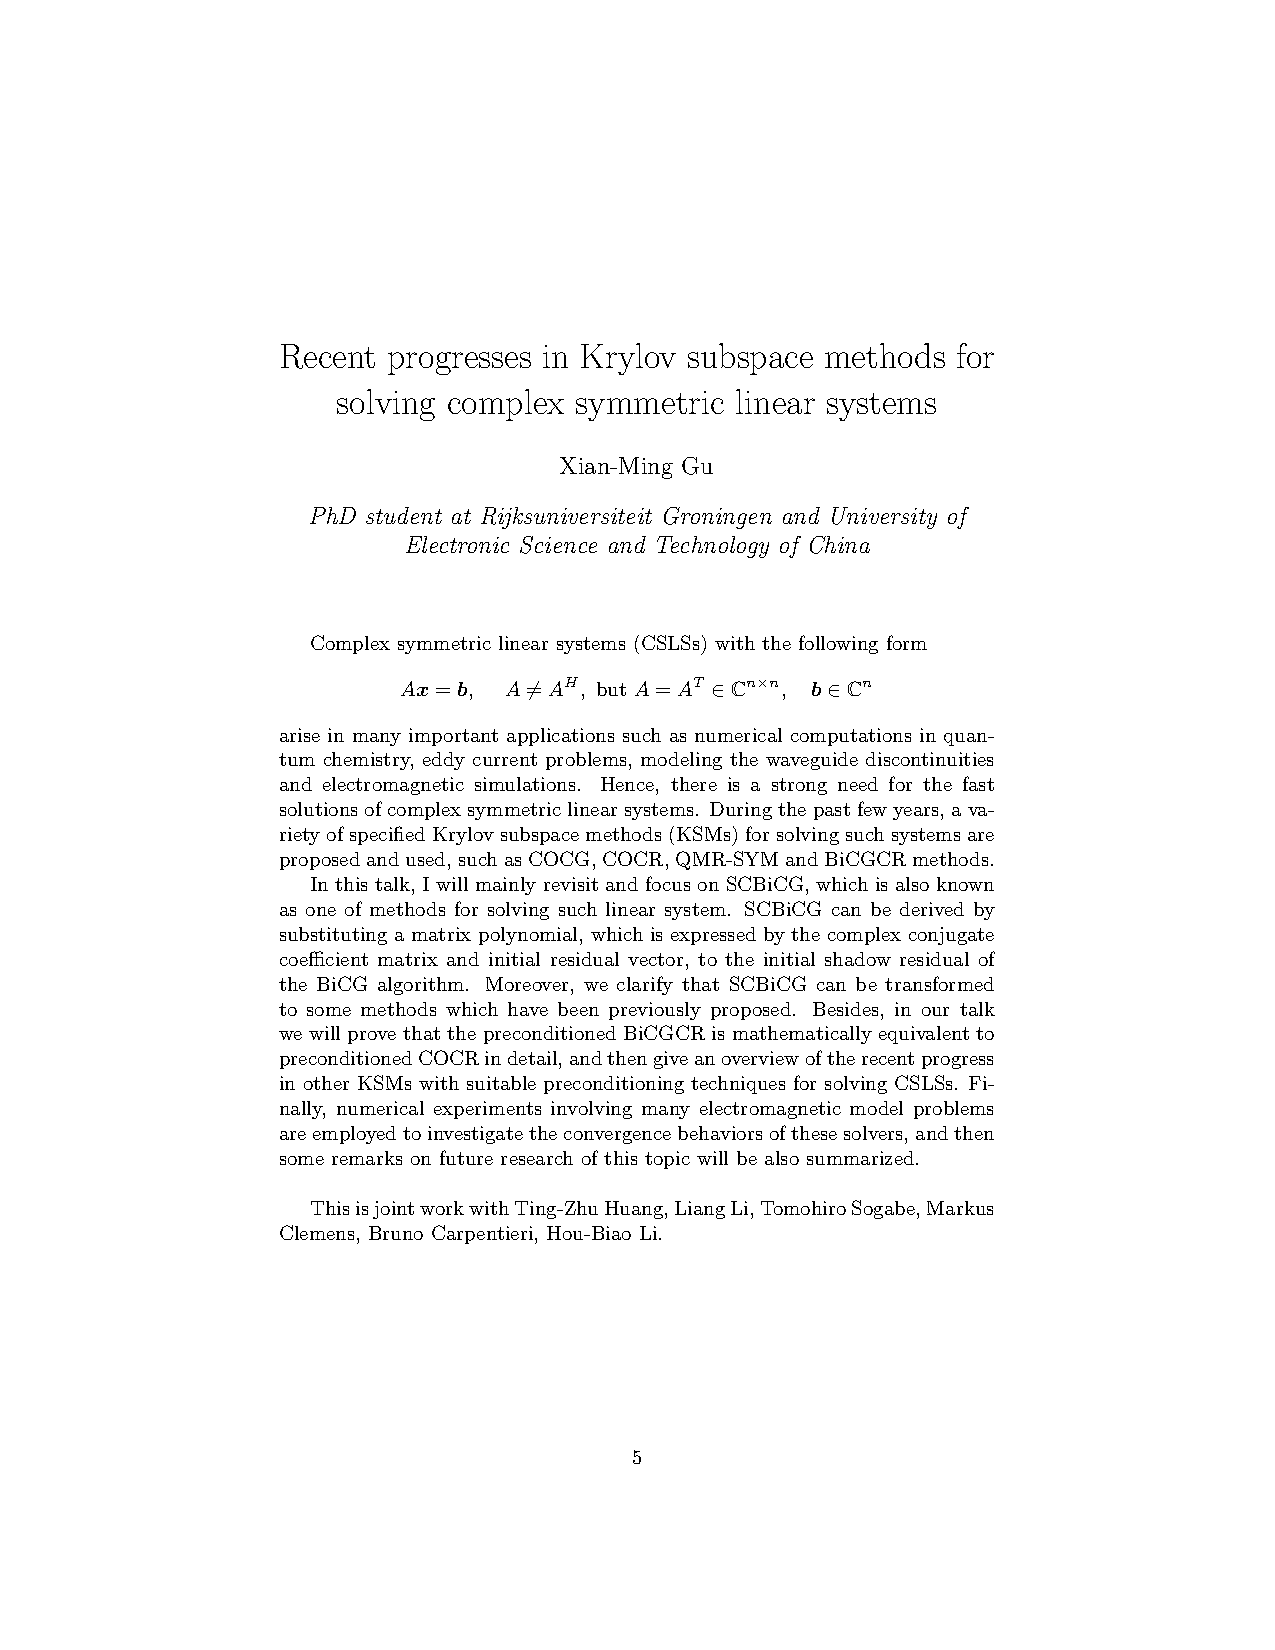
\includepdf[pages={1}]{abstracts/gu_kd_template.pdf}
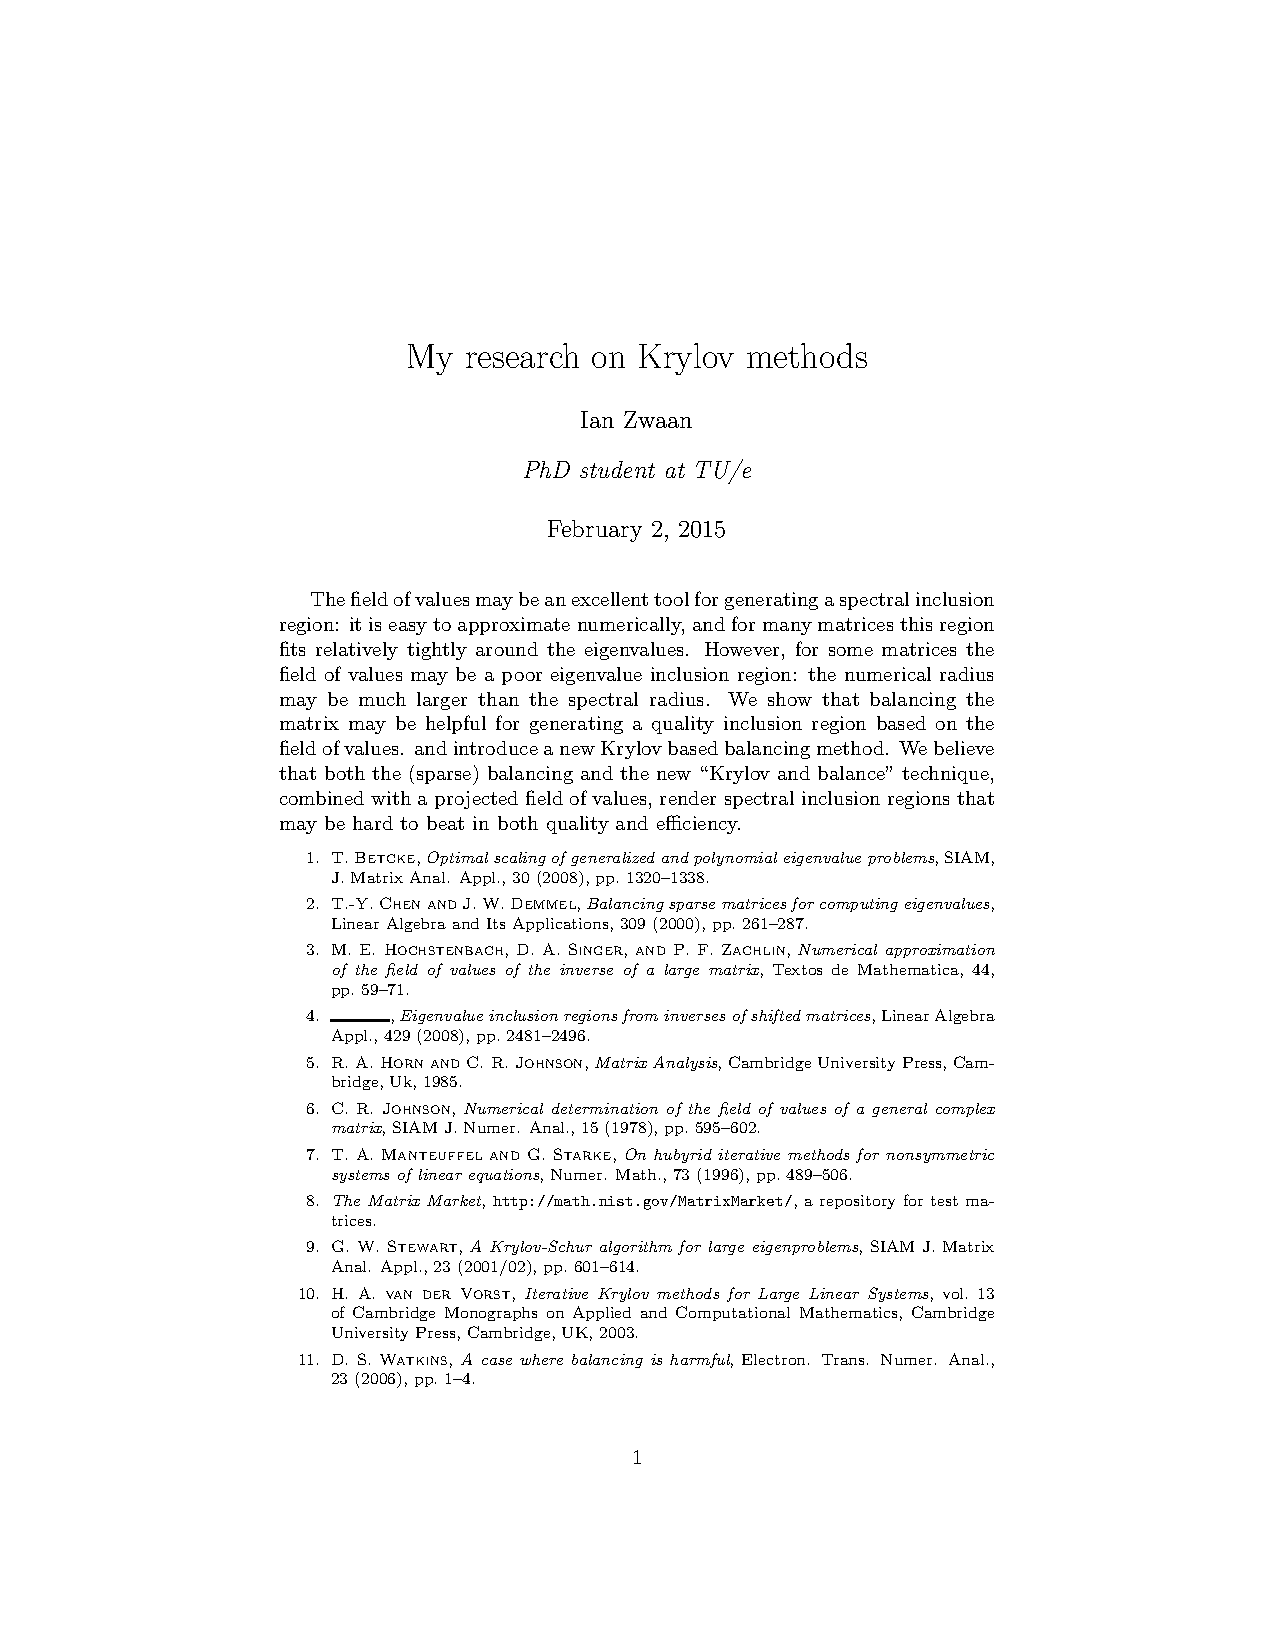
\includepdf[pages={1}]{abstracts/zwaan_kd15_template.pdf}
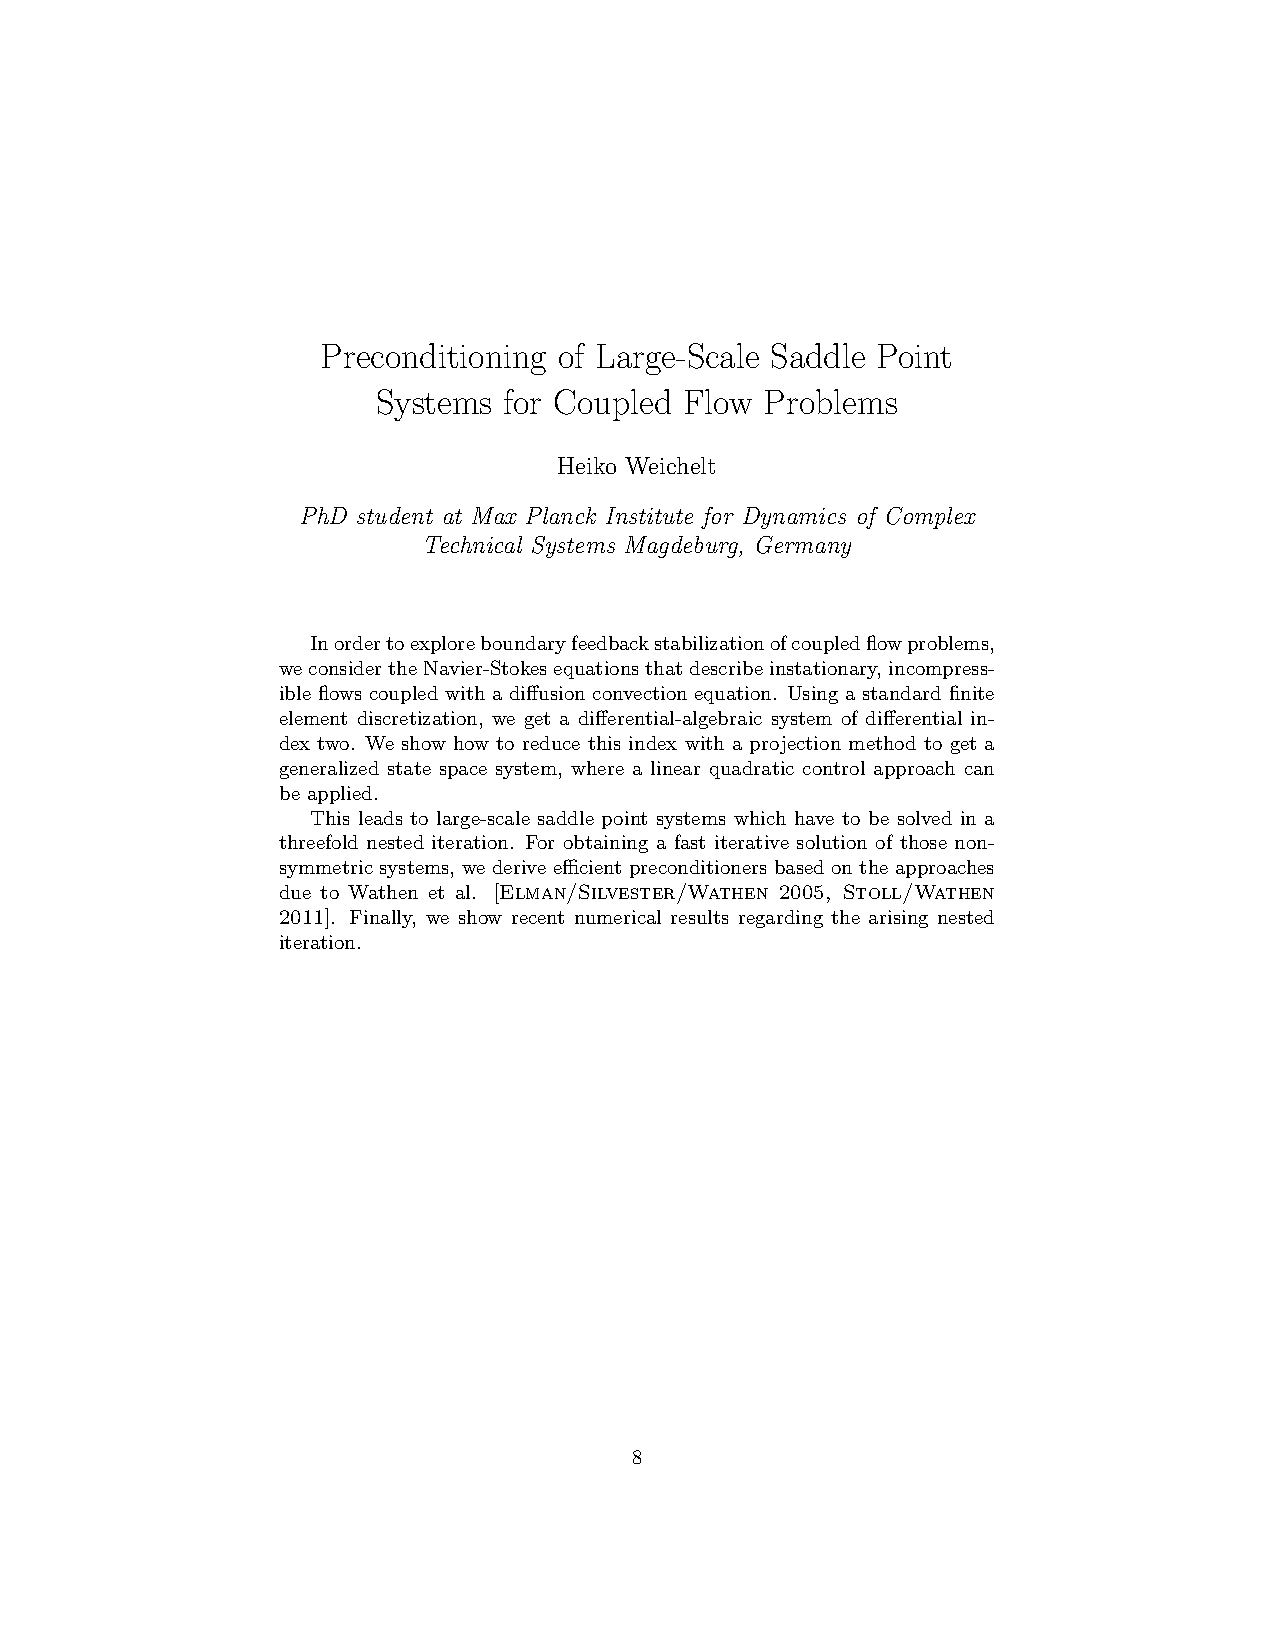
\includepdf[pages={1}]{abstracts/weichelt_abstract_KrylovDay_2015.pdf}
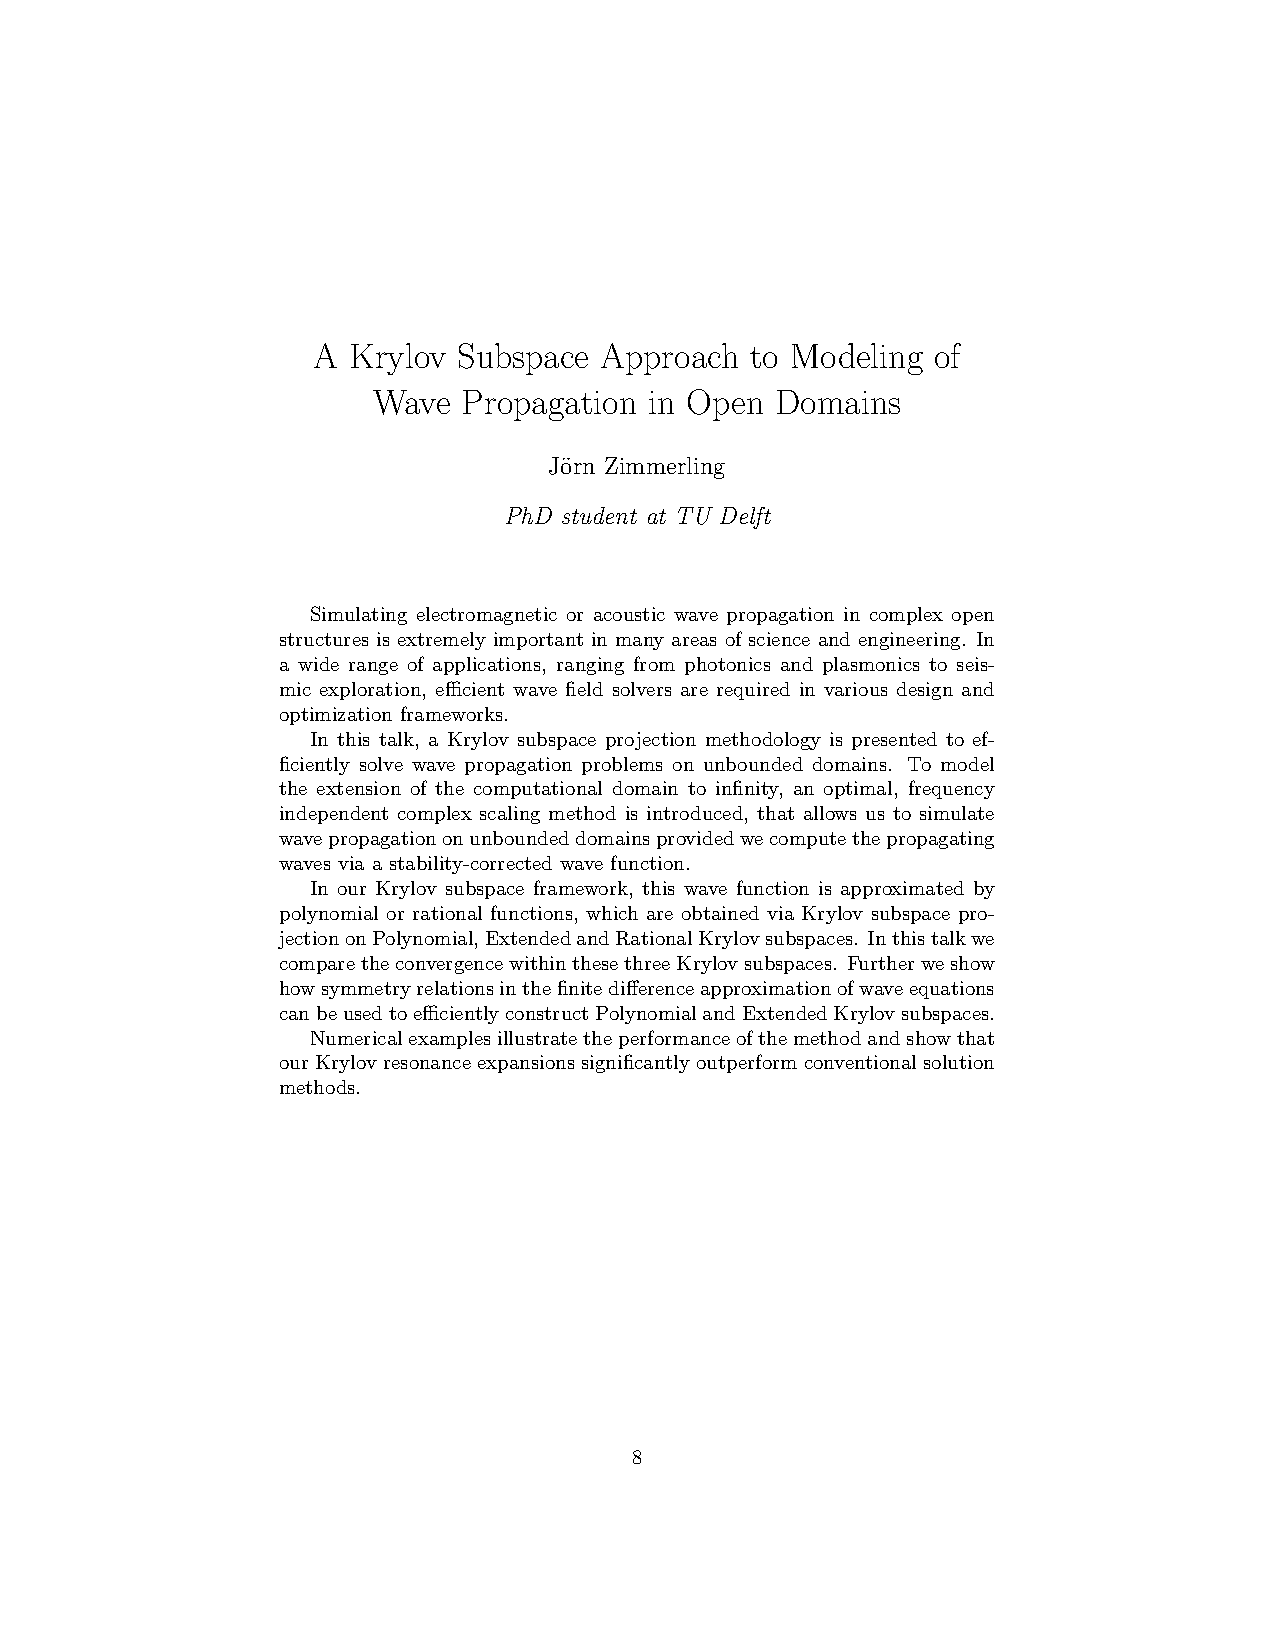
\includepdf[pages={1}]{abstracts/kd_jtzimmerling.pdf}
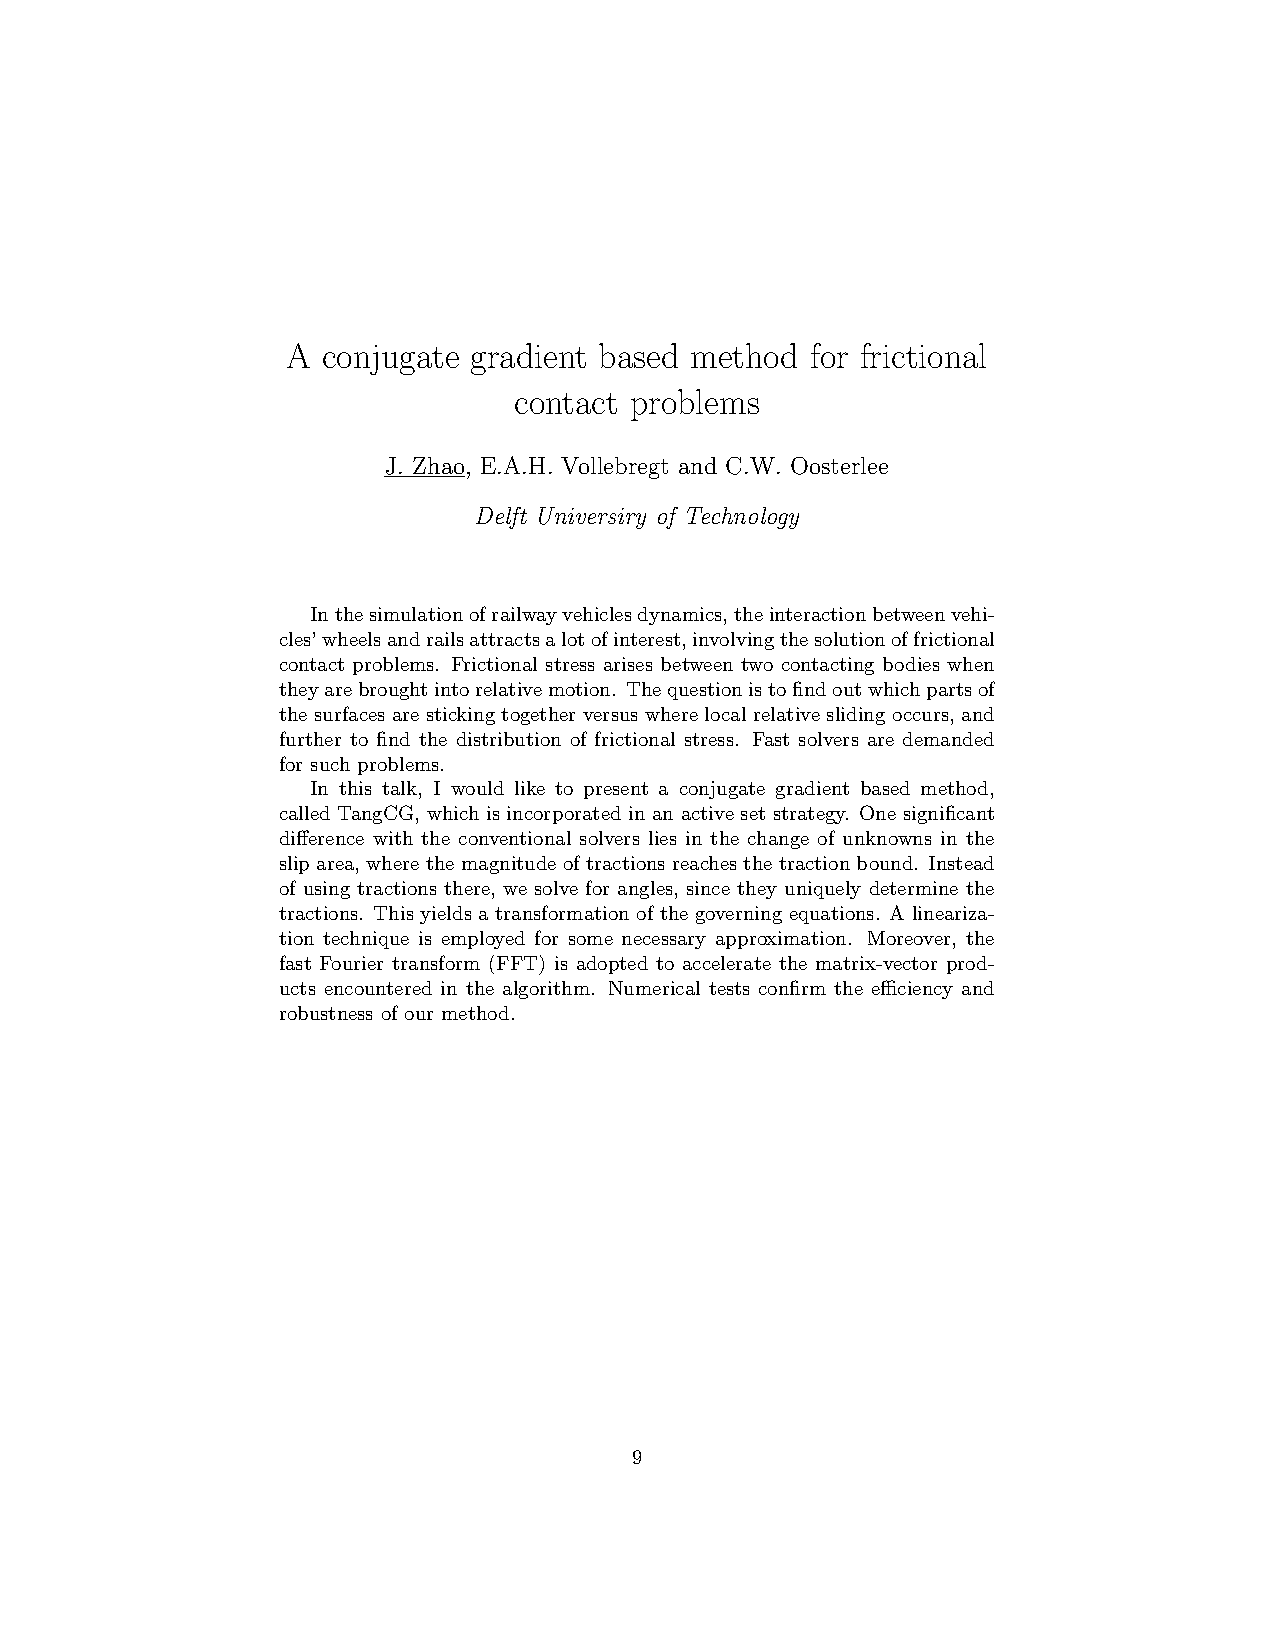
\includepdf[pages={1}]{abstracts/jing_kd_template.pdf}
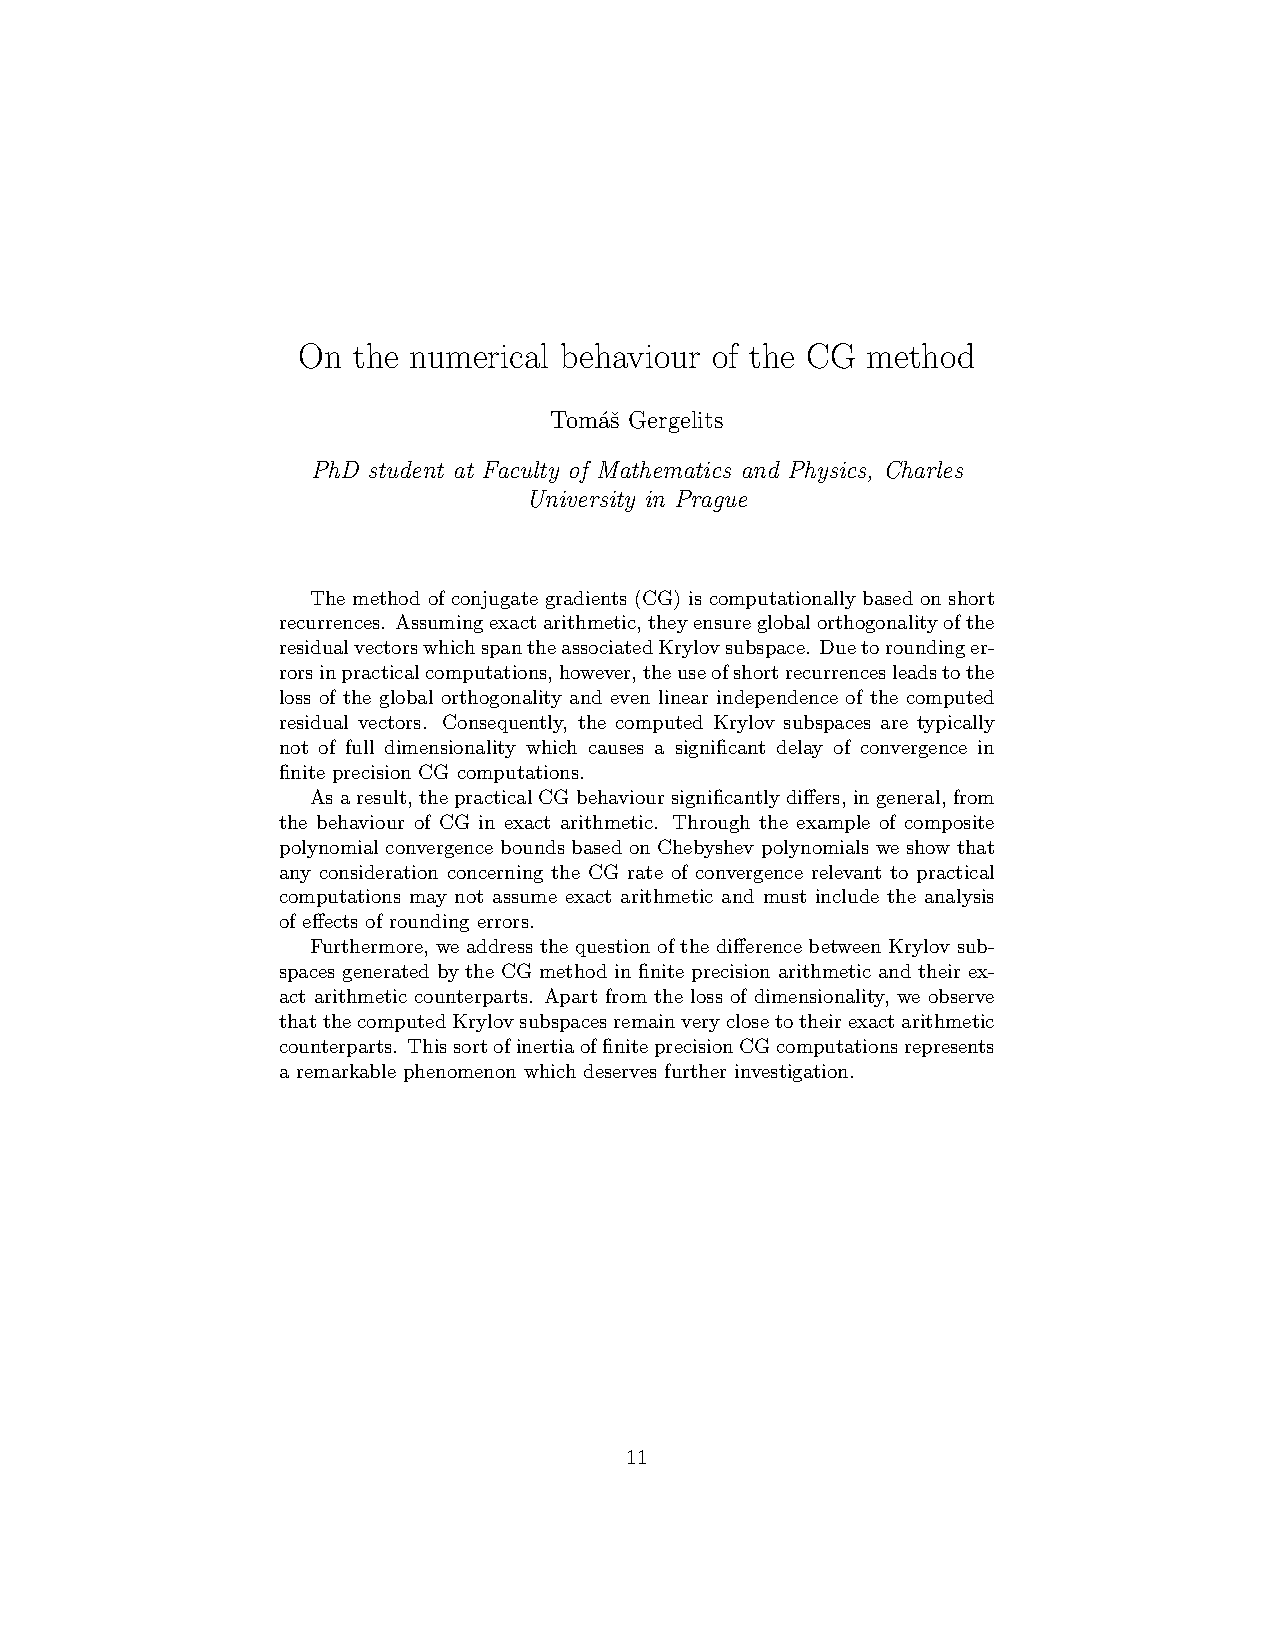
\includepdf[pages={1}]{abstracts/kd15_gergelits.pdf}
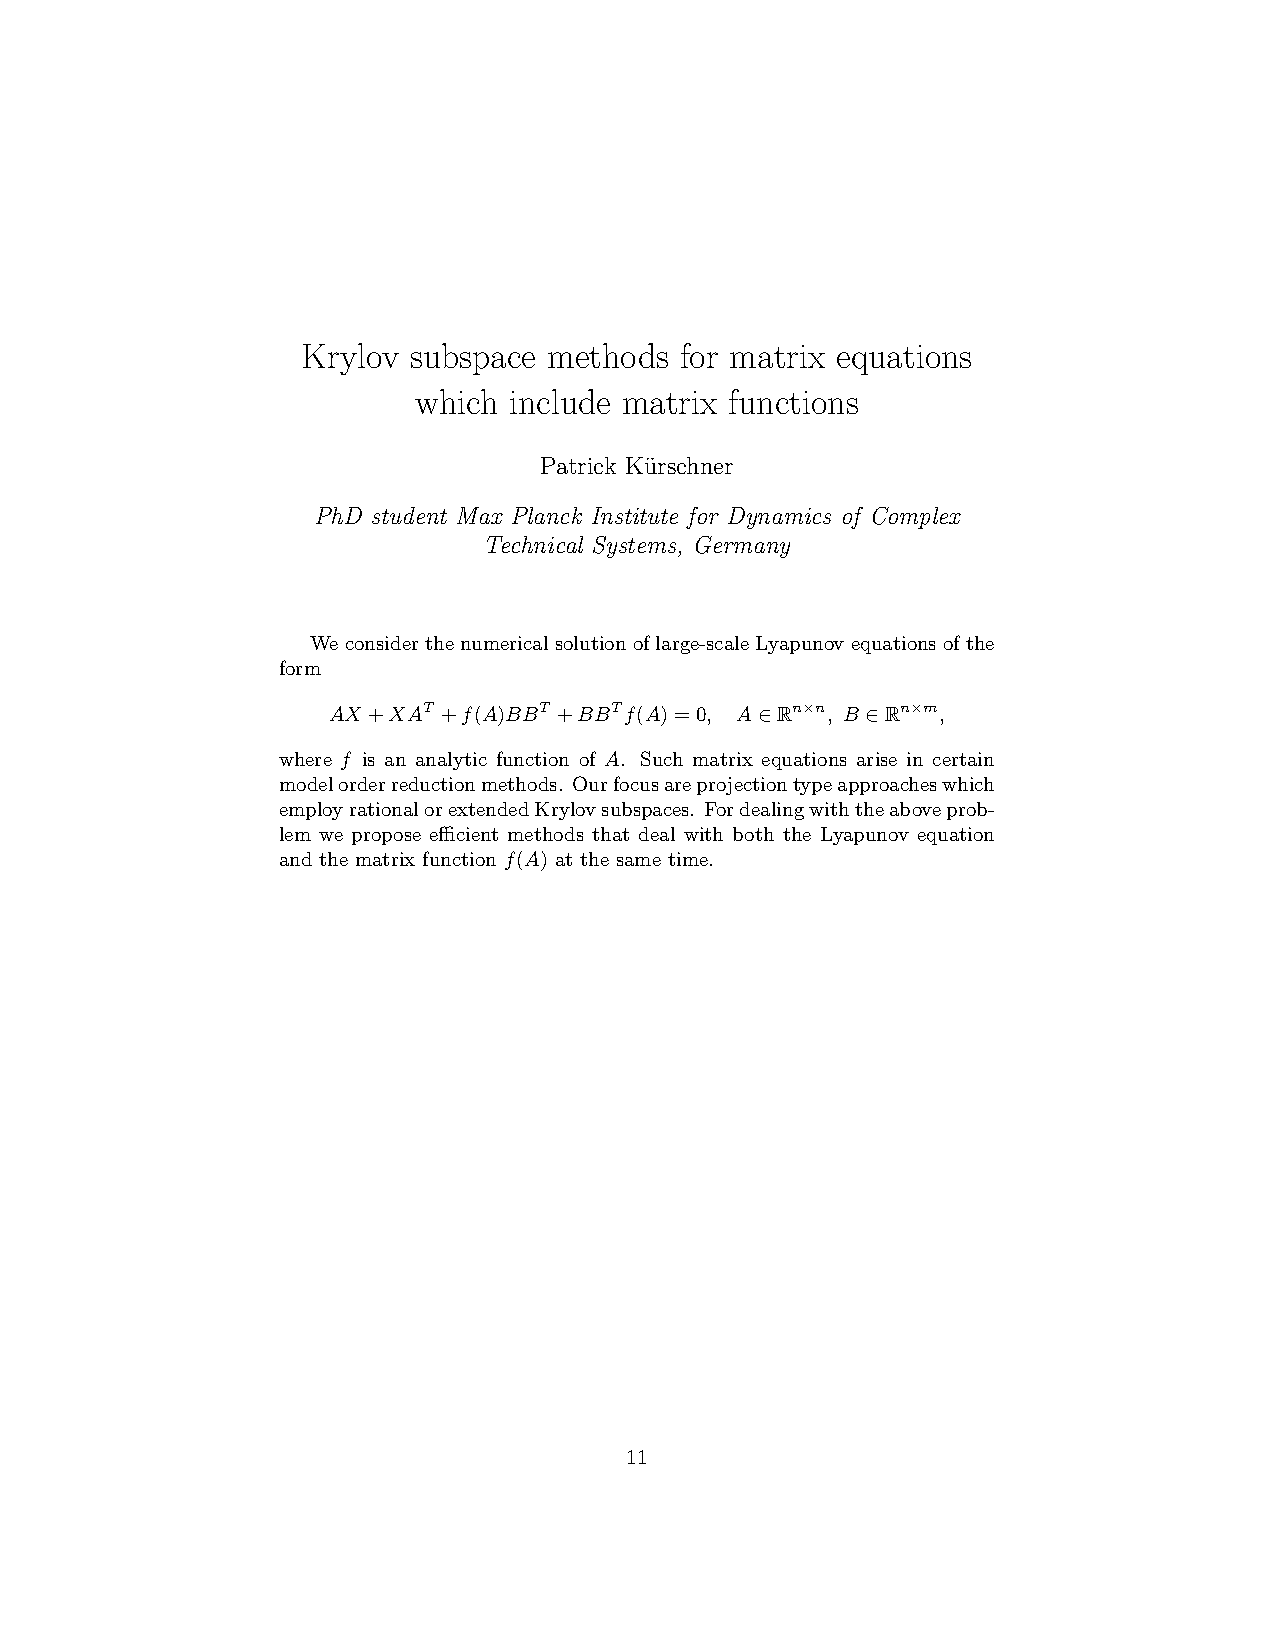
\includepdf[pages={1}]{abstracts/abstract_kuerschner.pdf}
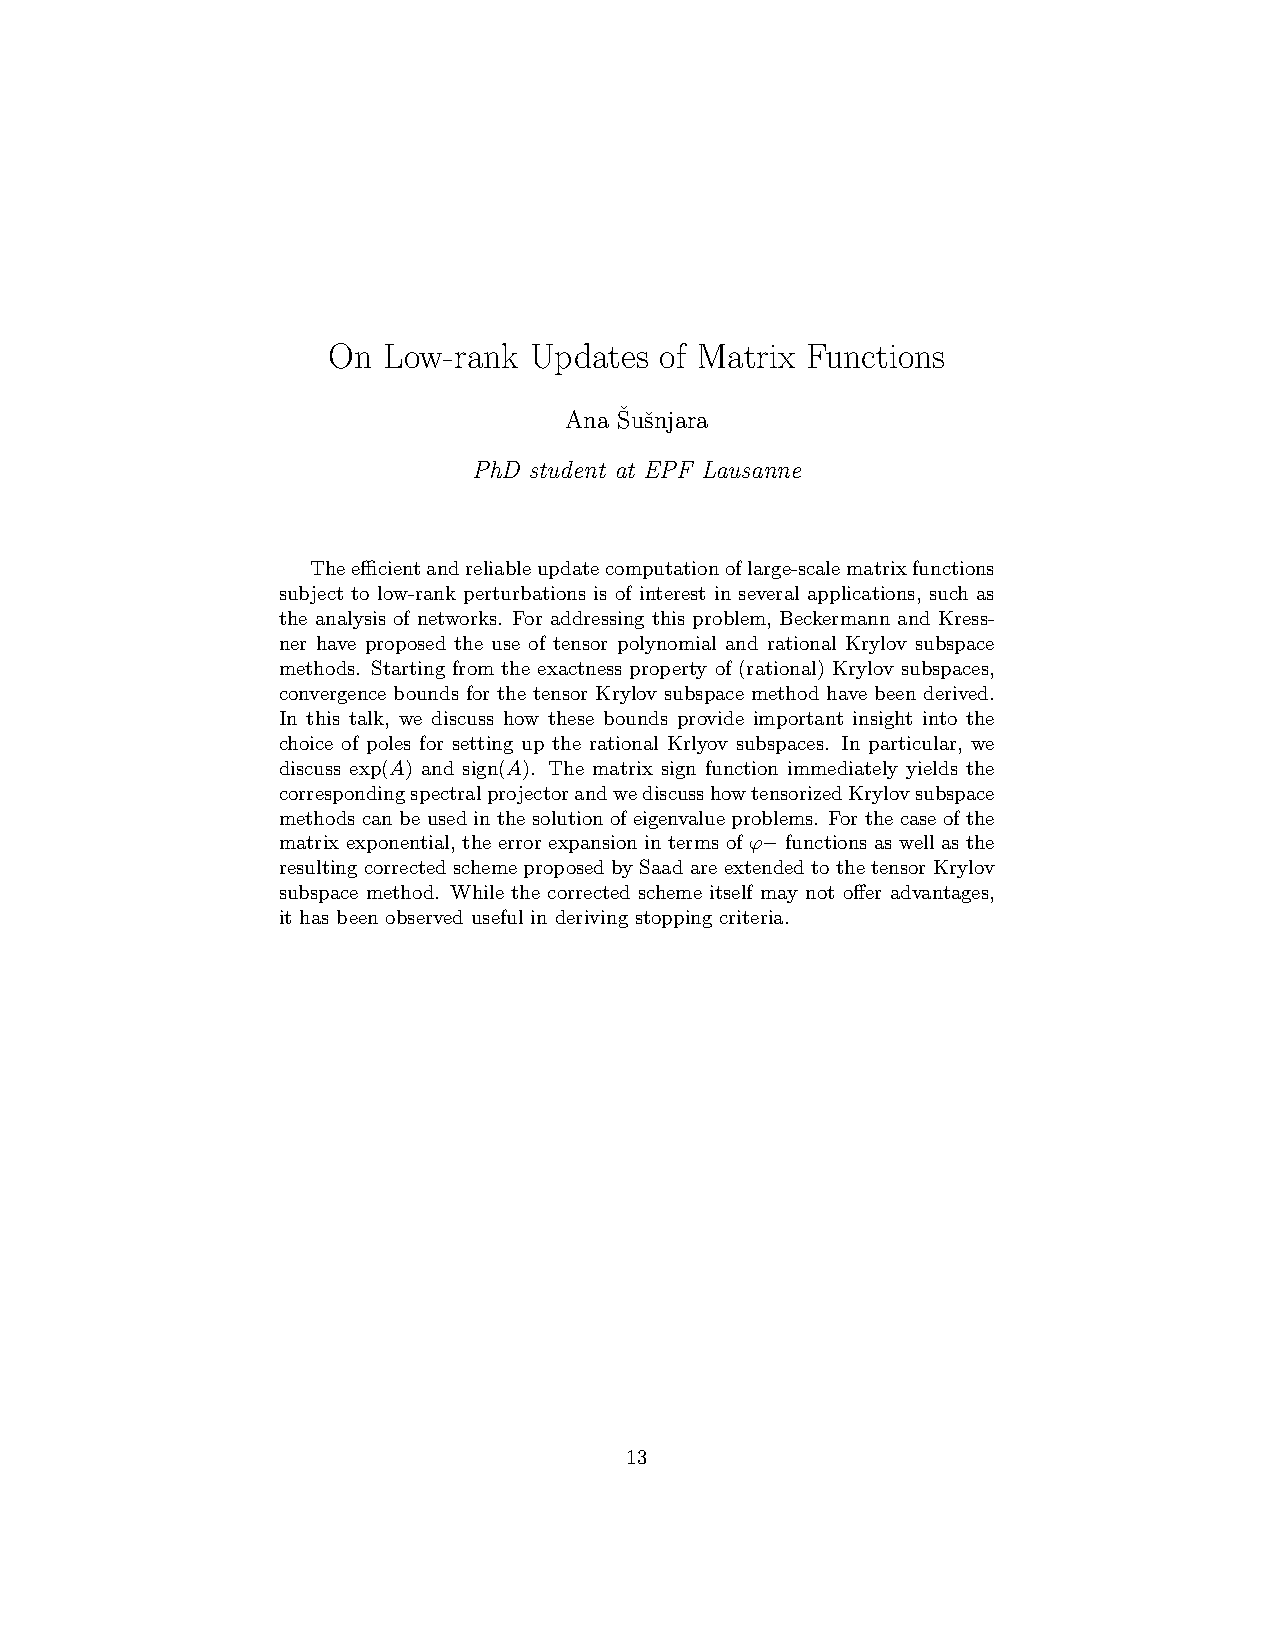
\includepdf[pages={1}]{abstracts/susnjara_template.pdf}
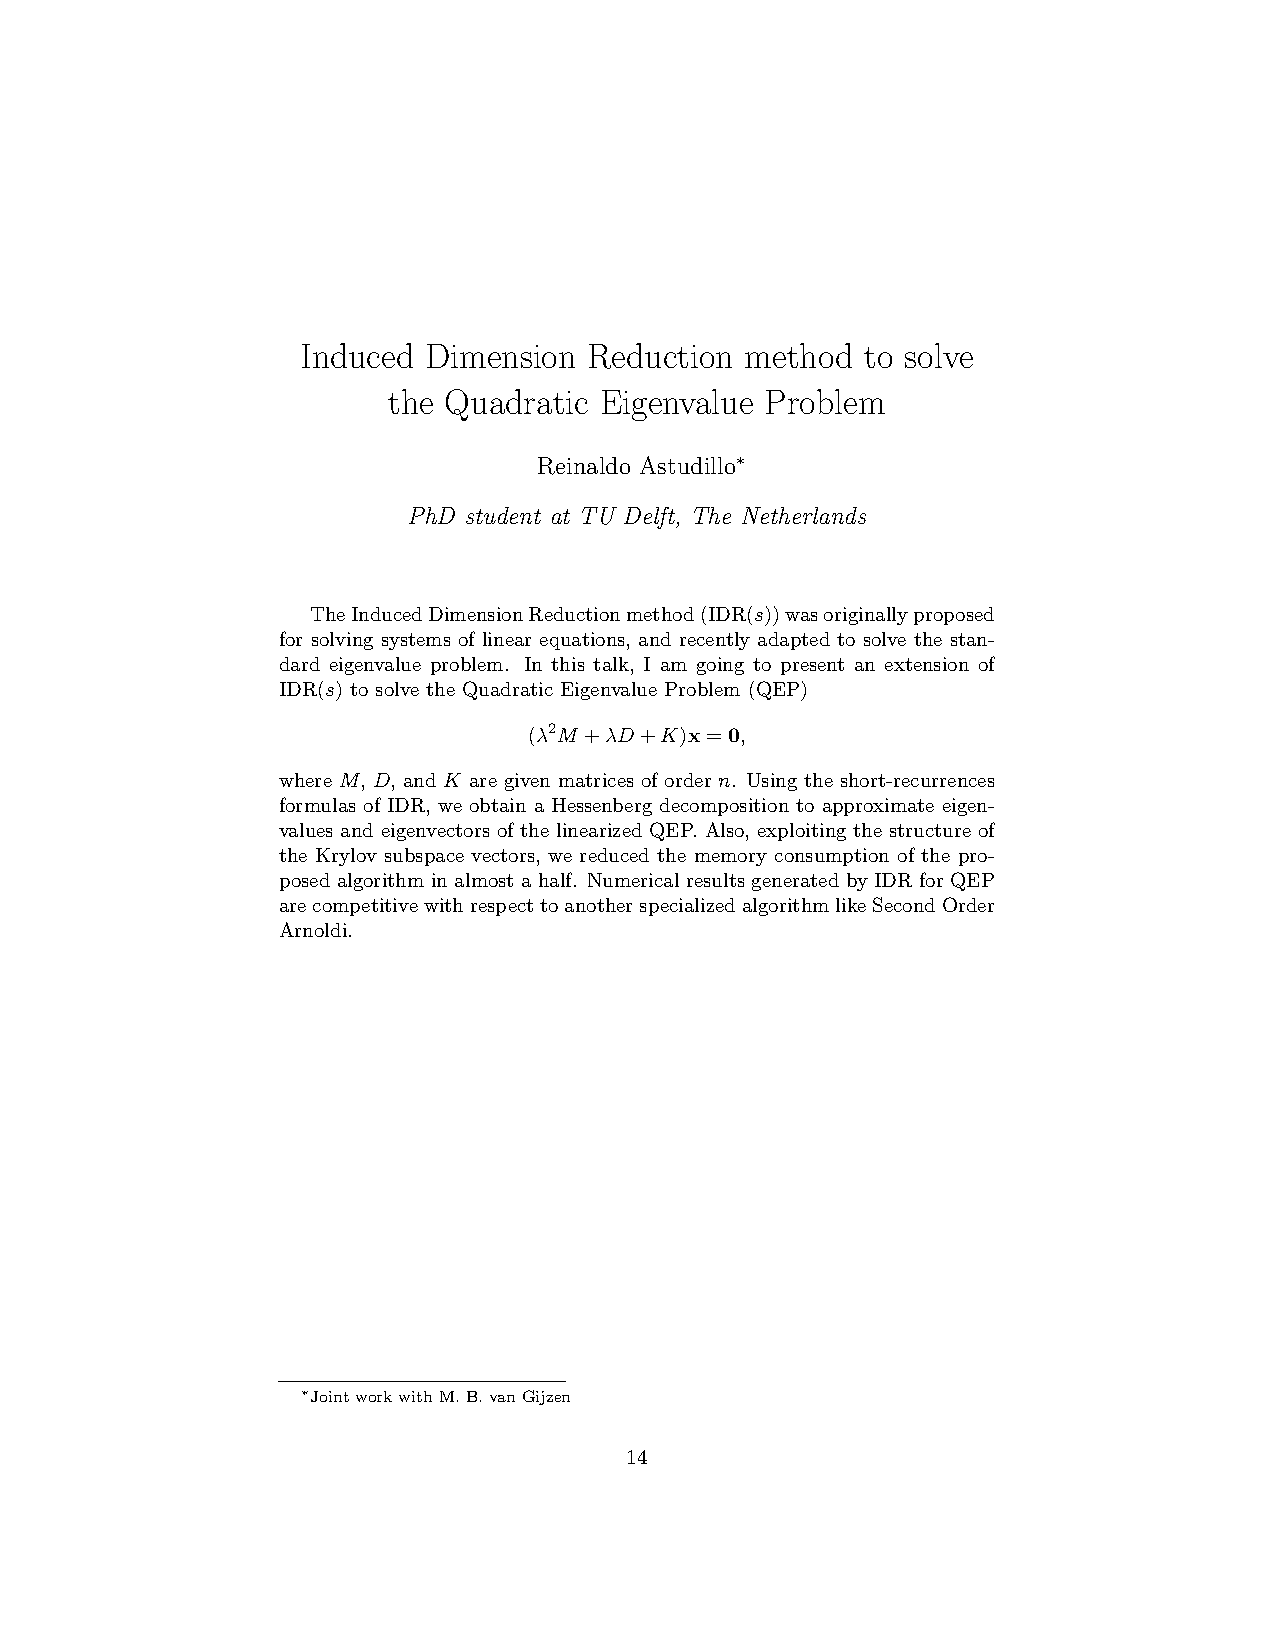
\includepdf[pages={1}]{abstracts/kd_template_Reinaldo.pdf}
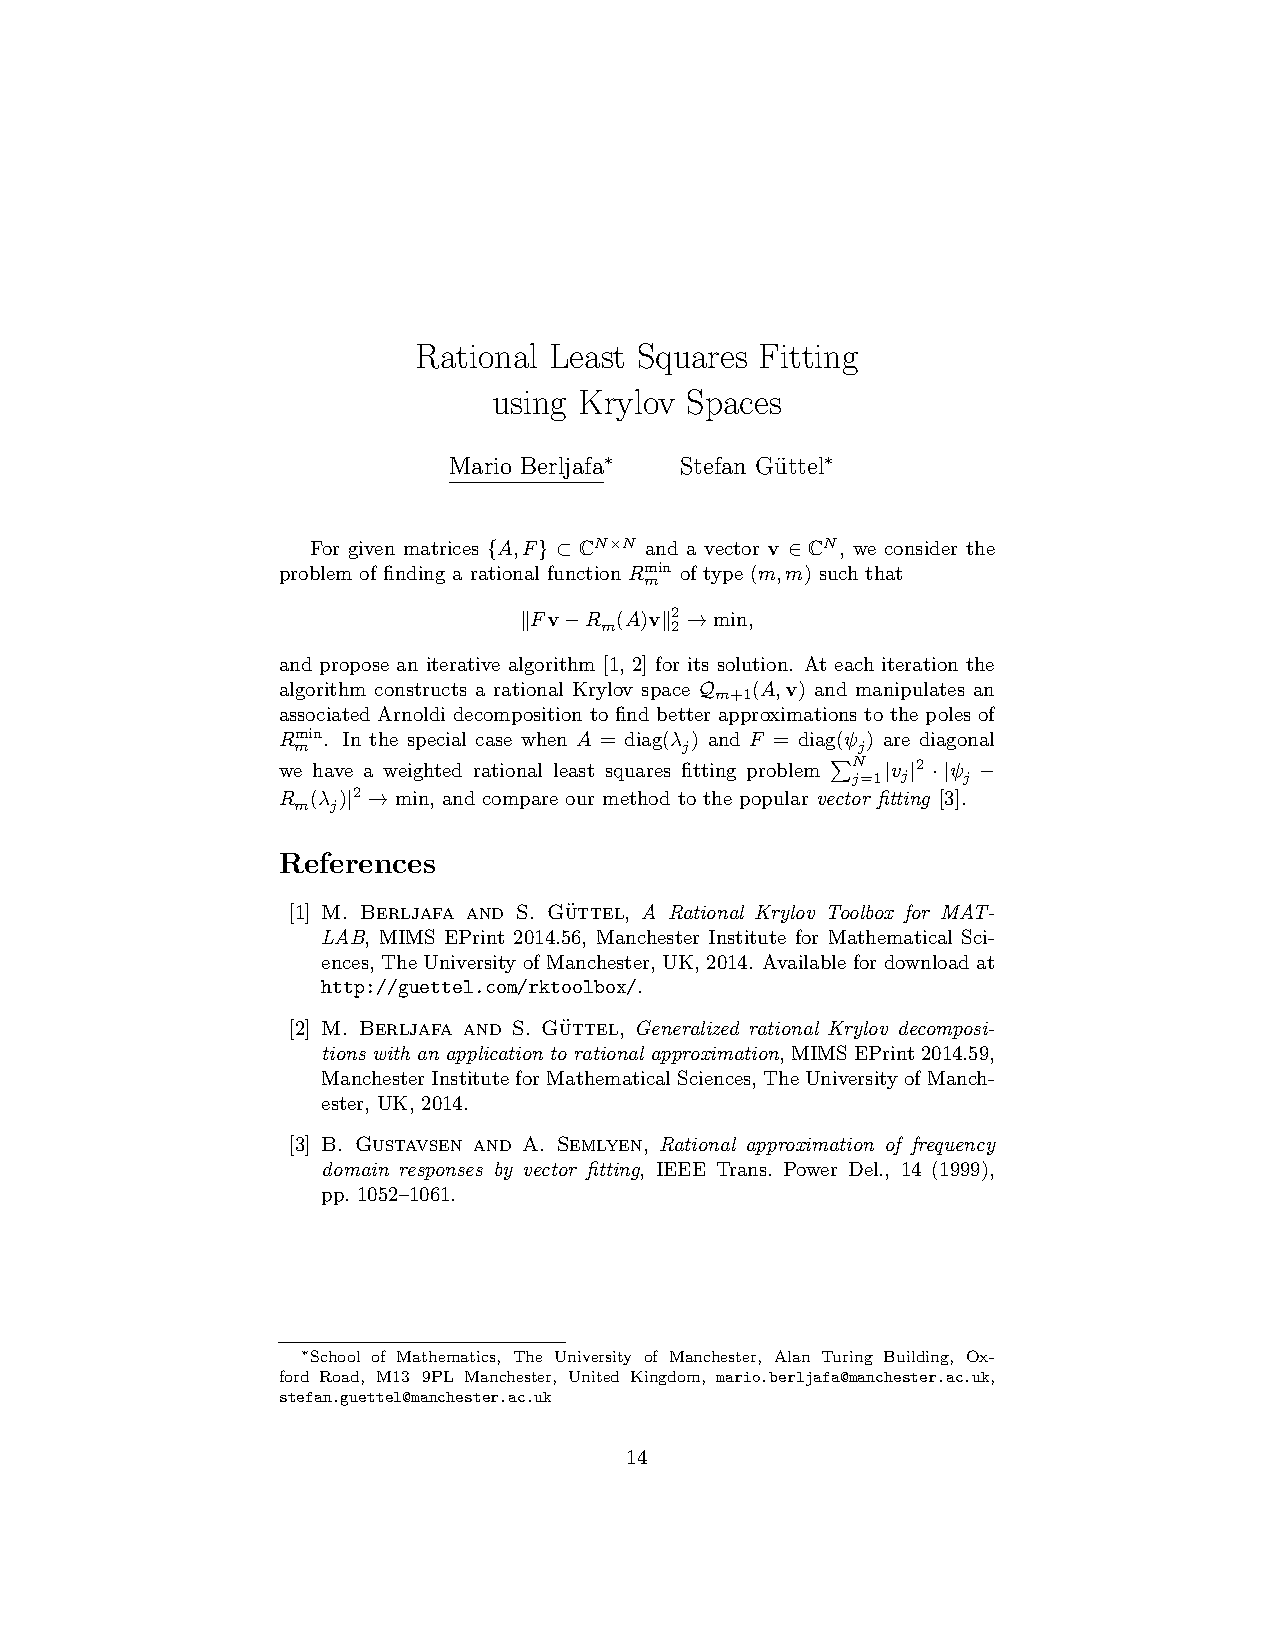
\includepdf[pages={1}]{abstracts/kd_berljafa.pdf}
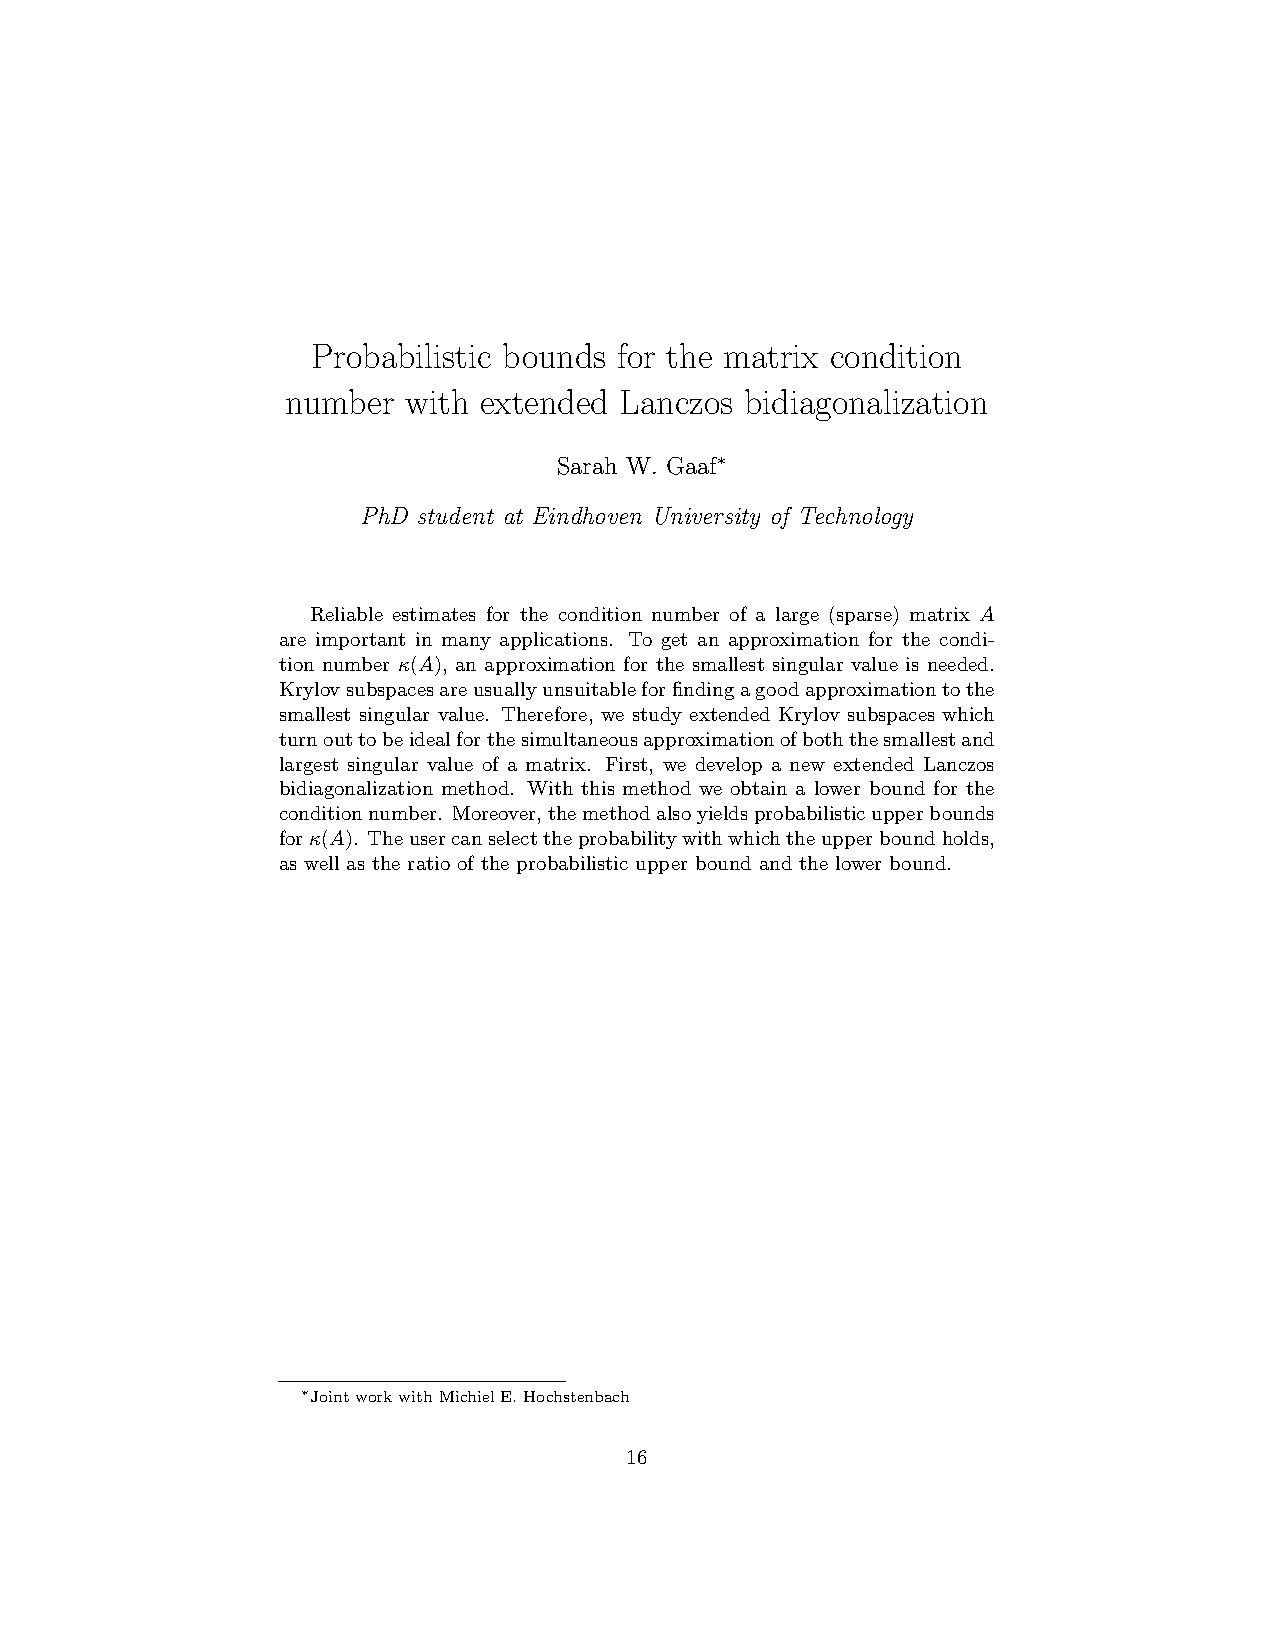
\includepdf[pages={1}]{abstracts/kd15_SarahGaaf.pdf}
\end{document}
